\title{Modular Deep Encoder-Decoders}
\author{Sebastien Arnold\Mark{1}, Prashanth Gurunath Shivakumar\Mark{2}, Cheng Qu\Mark{3}\\ and Qiangui Huang\Mark{4}}
%\affil[1]{Department of Computer Science, University of Southern California, Los Angeles, CA \authorcr Email: {\tt \{arnolds, chengqu, qianguih\}@usc.edu}\vspace{1.5ex}}
%\affil[2]{Ming Hsieh Department of Electrical Engineering, University of Southern California, Los Angeles, CA \authorcr Email: {\tt pgurunat@usc.edu} \vspace{-2ex}} 

\documentclass[12pt]{article}
\usepackage{amsfonts}
\usepackage{subcaption}
% Packages import
\usepackage[utf8]{inputenc}
\usepackage[T1]{fontenc}
\usepackage[english]{babel}
\usepackage{fancyhdr}
\usepackage{amsthm}
\usepackage{amsmath}
\usepackage{amssymb}
\usepackage{xpatch}
\usepackage{titling}
\usepackage{geometry}
\usepackage{multicol}
\usepackage{lipsum}
\usepackage{array}
\usepackage{algorithm}
\usepackage{algorithmicx}
\usepackage[noend]{algpseudocode}
\usepackage{listing}
\usepackage{graphicx}
\usepackage{longtable}
\usepackage{supertabular}
\usepackage{booktabs}
\usepackage{float}
\usepackage{hyperref}
\usepackage[export]{adjustbox}
\usepackage{breakcites}
\usepackage{color}
\usepackage{fancyvrb}
\usepackage{listings}
\usepackage{xcolor}

% Defining variables
\makeatletter
\let\Title\@title
\let\Author\@author
\let\Date\@date
\makeatother

% Margins
%\geometry{letterpaper, portrait, margin=1.00in}
%\geometry{legalpaper, portrait, margin=1.00in}
\geometry{a4paper, portrait, margin=1.00in, bottom=1.25in, top=1.25in}
 
% Headers and Footers
\pagestyle{fancy}
\fancyhf{}
\rhead{\Title}
\lhead{\Date}
\rfoot{Page \thepage}
\renewcommand{\headrulewidth}{2pt}
\renewcommand{\footrulewidth}{1pt}
\renewcommand{\qedsymbol}{$\blacksquare$}

% Section Customization
\renewcommand\thesection{{\Roman{section}}}
\renewcommand\thesubsection{}{\Roman{subsection}}
\renewcommand\thesubsubsection{}{\Roman{subsubsection}}

% Theorems and Tipps
\makeatletter
\xpatchcmd{\@thm}{\thm@headpunct{.}}{\thm@headpunct{}}{}{}
\newtheorem{theorem}{\underline{Theorem}}[section]
\newtheorem{definition}{\underline{Definition}}[section]
\newtheorem{corollary}{Corollary}[theorem]
\newtheorem{lemma}[theorem]{Lemma}
\theoremstyle{remark}
\newtheorem*{note}{Note:}
\theoremstyle{remark}
\newtheorem*{tip}{Tip:}

% Limit Image Width
\let\oldincludegraphics\includegraphics
\renewcommand{\includegraphics}[2][]{%
  \oldincludegraphics[#1,max width=\linewidth]{#2}}

% Code highlighting
\newcommand{\VerbBar}{|}
\newcommand{\VERB}{\Verb[commandchars=\\\{\}]}
\DefineVerbatimEnvironment{Highlighting}{Verbatim}{commandchars=\\\{\}}
\newenvironment{Shaded}{}{}
\newcommand{\KeywordTok}[1]{\textcolor[rgb]{0.00,0.00,1.00}{{#1}}}
\newcommand{\DataTypeTok}[1]{{#1}}
\newcommand{\DecValTok}[1]{{#1}}
\newcommand{\BaseNTok}[1]{{#1}}
\newcommand{\FloatTok}[1]{{#1}}
\newcommand{\CharTok}[1]{\textcolor[rgb]{0.00,0.50,0.50}{{#1}}}
\newcommand{\StringTok}[1]{\textcolor[rgb]{0.00,0.50,0.50}{{#1}}}
\newcommand{\CommentTok}[1]{\textcolor[rgb]{0.00,0.50,0.00}{{#1}}}
\newcommand{\OtherTok}[1]{\textcolor[rgb]{1.00,0.25,0.00}{{#1}}}
\newcommand{\AlertTok}[1]{\textcolor[rgb]{1.00,0.00,0.00}{{#1}}}
\newcommand{\FunctionTok}[1]{{#1}}
\newcommand{\RegionMarkerTok}[1]{{#1}}
\newcommand{\ErrorTok}[1]{\textbf{{#1}}}
\newcommand{\NormalTok}[1]{{#1}}
\lstnewenvironment{code}{\lstset{language=Haskell,basicstyle=\small\ttfamily}}{}


\newcommand\Mark[1]{\textsuperscript#1}

% Custom Title
\def\maketitle{
	\par\rule{\textwidth}{2pt}
	\par\hfill
	\begin{centering}
	\begingroup
	\centering
	{\par\textbf{\LARGE\@title}\\[1.5em]
	\large\par{\textit{\@author}}}\\[1em]
	\begin{tabular}{*{4}{>{\centering}p{.23\textwidth}}}
	\url{arnolds@usc.edu}\Mark{1} & \url{pgurunat@usc.edu}\Mark{2} & \url{chengqu@usc.edu}\Mark{3} & \url{qianguih@usc.edu}\Mark{4} \tabularnewline
	9013085897 & 2251924199 & 2385279985 & 9532576000
	\end{tabular}\par
	\endgroup
	\par\rule{\textwidth}{2pt}
	\end{centering}
}

\begin{document}
\thispagestyle{empty}
\maketitle
\hfill
\begin{abstract}
%In this short paper we propose an approach to transfer learning using rich
%vector embeddings. The suggested technique can be applied to any supervised
%task, and it handles multiple sources and changing sources of data without the
%need for retraining. To verify our ideas, we apply our ideas to the task of
%text-classification.

In this short paper, we propose a Modular Deep Encoder-Decoder network (MDED) for text classification. The basic idea behind MDED is to extend a pre-trained model, which consists of a set of deep encoder-decoders, with an additional source of data modality by adding a new encoder to the network. MDED has been applied to text classification on Saudi Newspapers Arabic Corpus (SaudiNewsNet). A modular Long Short Term Memory (LSTM) network is built. Experimental results show that our algorithm can efficiently combine new source of data and pre-trained model. The training process can converge into a local optimum in very few epochs when a new data source is added. With a good initial encoder-decoder, the modular LSTM networks can improve classification accuracy by up to 0.51\% when a new data source is added.

\end{abstract}

\section{Introduction}\label{introduction}

%Our goal is to generate rich vector embeddings from articles to classify
%them into predefined categories. Then, we want to extend our model with
%an additional source of data: the title of the videos. To handle this
%new knowledge source without retraining our previous model, we suggest
%to generate a new embedding that will be used to modify the original
%one. This combined embedding will then be used for the classification
%task.

In the past decade, deep learning has gained a lot of momentum in various fields. It has been successfully applied to natural language processing (NLP). End-to-end trained deep learning algorithms have been proven to outperform traditional algorithms on various NLP tasks. The success of deep learning is accounted for trading off computationally complexity for performance. The high complexity demand for training deep learning algorithms is inefficient especially when there is new complementary data modality to be used to update a model and re-train it from scratch every time. To alleviate this problem, a novel Modular Deep Encoder-Decoder network (MDED) is proposed in this paper. The basic idea behind MDED is to extend a pre-trained model, which consists of a set of deep encoder-decoders, with an additional source of data modality by adding a new encoder to the network. 


More formally, we want to jointly learn a set of \emph{encoder}
functions $\{E_i\}_0^N$ mapping samples $x \sim \chi_i$ from a set of
data distributions $\{\chi_i\}_0^N$ to a fixed-sized vector embedding
$V$.

\[ \forall i \in [0; N]: E_i(x): \chi_i \rightarrow V_i \in \Re^M\]

\[V = \sum_i^N V_i\]

The embedding $V$ is then fed into a decoder function $D$ which in the
case of classification learns a mapping from the vector space of $V$ to
the label space $L$.

\[ D(v): \Re^M \rightarrow L \in \Re^D\]

Finally, we want to extend the set of encoders by learning a new encoder
$E_{N+1}$ which handles samples from a different dataset $\chi_{N+1}$,
without retraining our trained decoders and encoders.

\[ E_{N+1}(x): \chi_{N+1} \rightarrow V_{N+1} \in \Re^M\]

\begin{figure}[htbp]
\centering
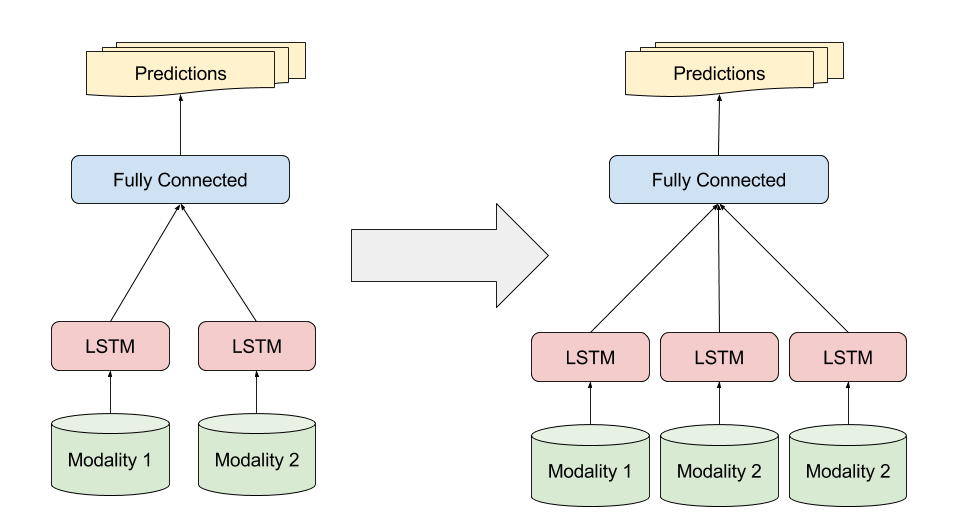
\includegraphics[width=0.5\textwidth]{figures/multimodal.png}
\caption{Multi-modal Transfer Learning}
\end{figure}

Although we could have used any kind of mapping, we chose to use deep
learning algorithms, as they easily learn hierarchical representations
and have been known to highly outperform other statistical techniques on
natural language tasks. Learning embeddings has been previously done by Zhuang \& al in 
\cite{zhuang2015supervised}, although our proposed contribution is
slightly different. They used deep autoencoders to
obtain a better initialization of the parameters of their model. Our
approach instead is much closer in spirit to the work of Sutskever \& al
\cite{sutskever2014sequence} and Vinyals \& al \cite{vinyals2015grammar}. They
both use encoders on a sequence of data to generate a
\emph{thought-vector} which will then be decoded in the desired target
sequence. In some sense, our proposal adds the transfer learning
component to their contribution. This approach is also similar to the
work of Karpathy \& al \cite{karpathy2014deep} where they mapped
images to their captions with embeddings.

In this paper, we evaluate the effectiveness of idea by applying the concept towards a simple NLP classification task. We adopt Saudi Newspapers Arabic Corpus \cite{hagrima2015} to classify text into different journals based on the article content, author and title.

\section{Method}\label{method}
\subsection{Materials}
\subsubsection{Corpora}
We use the freely available Saudi Newspapers Arabic Corpus \cite{hagrima2015}. The dataset contains a total of 31,030 Arabic newspaper articles, with a total number of 8,758,976 words. 

\begin{figure}[h!]
\centering
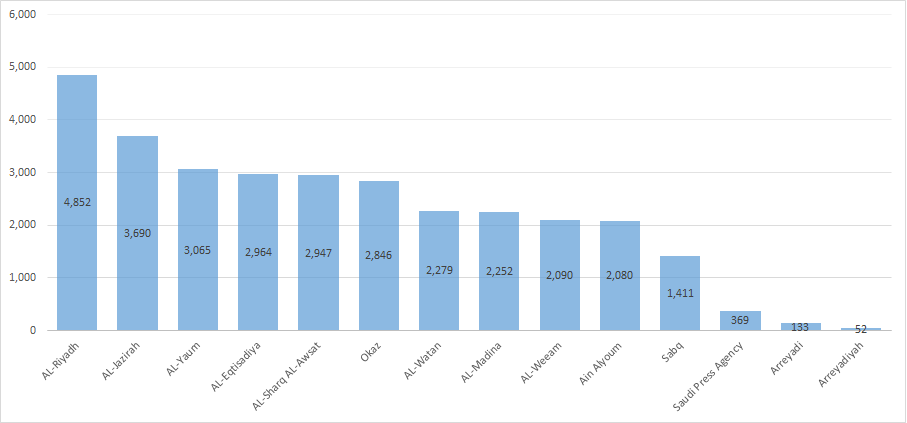
\includegraphics[width=0.65\textwidth]{figures/article-newspaper_distribution.png}
\caption{Figure shows article-newspaper distribution}
\end{figure}

Article objects are represented in json format, with UTF-8 encoding. We wrote a script to download the data from github repo, unzip each file, and read them in as json objects. Each json object contains the following fields:

\begin{itemize}
\item source: A string identifier of the newspaper from which the article was extracted.
\item url: The full URL from which the article was extracted.
\item date\_extracted: The timestamp of the date on which the article was extracted. It has the format YYYY-MM-DD hh:mm:ss. 
\item title: The title of the article. 
\item author: The author of the article.
\item content: The content of the article.
\end{itemize}

% This picture is not relevant to us
%\begin{figure}[h!]
%\centering
%
\includegraphics[width=\textwidth]{figures/title_example.png}
%\caption{An example of an article title}
%\end{figure}

The dataset is partitioned into training, development and testing subsets. 80\% of the data is assigned for training and 10\% for development and testing. The development set is utilized for hyper-parameter tuning and the results are finally presented on the testing set. During partitioning, care is taken to ensure appropriate percentage of data is seen in all the classes. Figure~\ref{fig:dist} shows the distribution of data used for training and testing in each class. Figure~\ref{fig:sent_dist} shows the distribution of sentence lengths of the content of the articles.

\begin{figure}[h!]
\centering
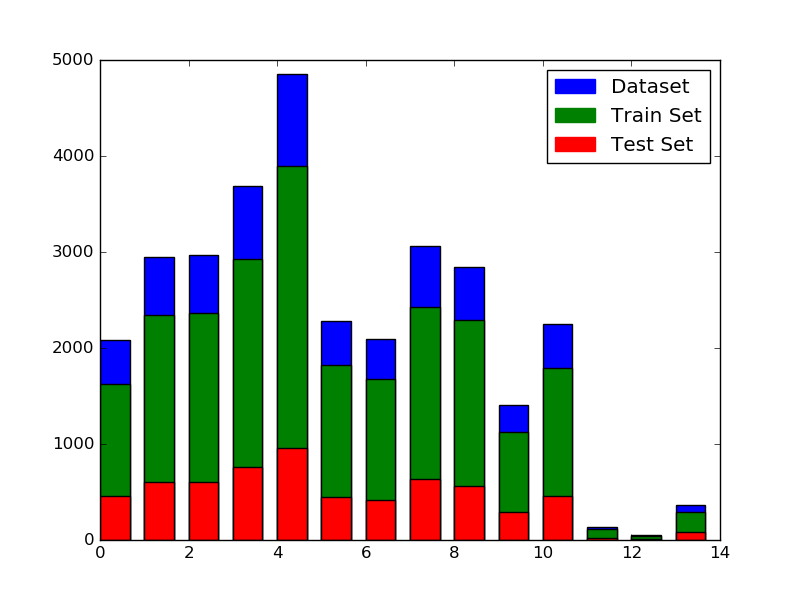
\includegraphics[width=0.65\textwidth]{figures/test_class_distribution.png}
\caption{Distribution of data for training and testing}\label{fig:dist}
\end{figure}

\begin{figure}[t]
\centering
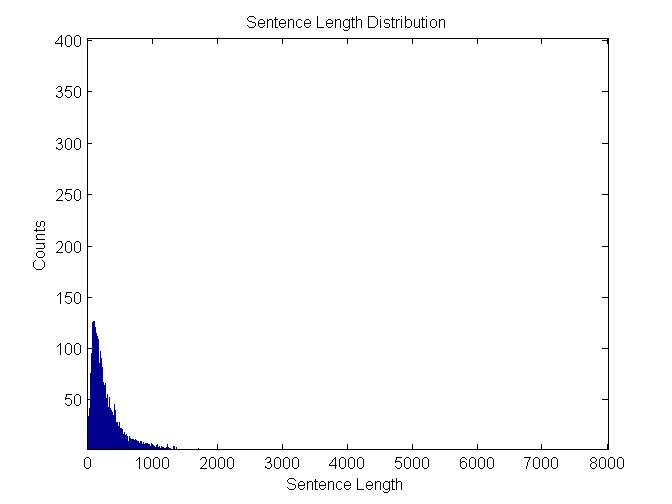
\includegraphics[width=0.65\textwidth,height=6cm]{figures/sentence_length.png}
\caption{Distribution of data for training and testing}\label{fig:sent_dist}
\end{figure}

\subsubsection{Tools}
For training the neural networks, the neon toolkit was employed \cite{Neon}. Neon is Nervana's python based deep-learning library. The toolkit was chosen because of its flexibility of training on both CPU and GPU, its good support for neural network components, and it's state-of-the-art performance on GPU. In addition, one of the team members is a core contrubtor to the framework.

\subsection{Procedure}\label{procedure}

\subsubsection{Data Pre-processing and Features}

Firstly, the UTF-8 encoded data was checked for trailing spaces for removal. Next, the data was filtered by removing punctuation symbols, retaining only a subset consisting of \{$,$ $.$ $!$ $($ $)$ $?$\}. The data was then split into words which are used as tokens for building the vocabulary and finally obtaining a feature representation for training the neural network. A vocabulary is constructed by assigning unique integer word-ids to each unique word appearing in the corpora. The punctuations are treated as a separate token and contributes to the vocabulary. The url, date and title fields of the corpora were discarded since they were irrelevant for our purpose.  

After building the vocabulary for the corpora, the original sentences of the corpora are mapped on a word-basis to obtain a series of integers representing the sentence equivalent which form the features to be input to the embedding layer of the neural network. Alternatively, the integer mapping could be replaced with one-hot sparse encoding of each word constituting the sentence. The features are shuffled and split for training and testing. For efficient data storage and retrieval the features are compressed to HDF5 file format.

\subsubsection{Embedding Layer}
An embedding layer is used to compute a word embedding $W: words \mapsto \mathbb{R}^{n}$ which is a function mapping words of a language to a high dimensional vectors which are continuous, distributed representation of the vocabulary words with good semantic properties. The hope of such a representation is to project similar words to similar regions in the hyper-space from a semantic point of view. 

%\subsubsection{Discriminative Model}

\subsubsection{Baseline System}
We construct two baseline systems, one to classify the journals based on the
content of the articles and the second on their authors. Identical architectures are used for both the baseline
systems. The encoder of the baseline system is a recurrent neural network with one hidden Long Short Term Memory (LSTM) layer succeeding the embedding layer. The dimension of both the embedding layer and the LSTM was fixed to 128. The decoder is a softmax layer with 14 outputs, one per class. The model minimize a cross-entropy loss using adaptive gradient descent \cite{duchi2011adaptive}. 

\subsubsection{Proposed System}
Once the baseline encoder and decoder have been trained on a single modality, we serialize their parameters on disk. We then proceed to the augmentation of our model by adding a new encoder. We first jointly load both modalities from the dataset - in our case the authors and the content of the articles - as well as their targets. We then instanciate two encoders and one decoder with random initialization. The parameters of the decoder and of one of the encoder are set from the serialized values obtained from the baseline. We then proceed by training our augmented model on both modalities. To ensure that the parameters of the initial encoder are not changed, we manually set the scaling factor of the gradients to zero. This results in the backpropagated errors - the partial derivatives of the errors with respect to the inputs - to be zero and the adaptive gradient descent step to have no effect.

Both of the encoders use an identical structure independently of the modality they are trained on. This model architecture is identical to the one described in the baseline system subsection.

We tried two approaches when building the vector embedding from multiple modalities. The first one was to vertically stack the different embeddings from the different encoders and learn the actual embedding as a linear combination from this higher dimensional vector. This led to poor results and we instead decided to experiment with both the summing over every embedding, as well as taking their mean in each dimension. Both approaches resulted in fairly similar results, however and we decided to use the mean of the embeddings in our experiments. The intuition behind this decision is grounded in the observation that taking the mean of several embeddings will have a less drastical effect on the decoder, thus stabilizing the learning in early stages of the transfer training.

\subsubsection{Hyper-parameter Tuning}
Using the development set, the hyper-parameters were fine-tuned for better performance. The tuning of sentence length cut-off for training the embedding layer was found to be critical especially when training on the content of articles. Setting lower sentence length resulted in over-training of the system. The distribution of the sentence lengths were plotted as shown in Figure~\ref{fig:sent_dist}. Looking at the distribution, we found the value of 2048 to be optimal. Different values for learning rate, hidden-layer dimensionality and non-linearity were experimented. Through a series of experiments, we found the optimal setting for initial learning rate is 0.01, optimal hidden-layer dimensionality is 128, and tangent function is the optimal activation function in hidden layers.


%The procedure is quite straight-forward. While part of the team worked on
%building our tailored dataset, the other half worked on the model definition
%and training procedure.

%Once every pre-requisite is available, we trained the first encoder $E_1$
%(implemented as a recurrent neural network) to build the embedding $V_1$. Since
%we only dealt with a relatively simple classification task, our decoder $D_1$
%was simply a fully connected multi-layer perceptron. They were jointly trained
%end-to-end by propagating the gradients through the embedding from $D_1$ to
%$E_1$.

%The second training step was to train the second encoder $E_2$. Again, we also
%performed training end-to-end, but specifically did not propagate the gradients
%through $E_1$.

\subsection{Evaluation}
The evaluation procedure for all experiments is based on the classification accuracy of each statistical model on a held-out test data. Meanwhile, we identify that the accuracy is not an ideal evaluation criteria considering the skewed nature of class distribution. To get a more meaningful representation of the performance F1-score or AUC metrics will be provided in the future work. However we stress the validity of the accuracies provided in the results section by comparing it to the random baseline. Taking into account the multi-class (14 class problem) nature of the classification and the prior for each class, we would like to point out that the average accuracy or chance accuracy of the data is 9.68\% which forms the random baseline of the problem under investigation.


\section{Results}\label{results}

\subsection{Baseline System}

First, three single LSTM networks are trained for text classification, where title, author and content values are used for training data, respectively. The hyper-parameter setting is same as introduced in above section. The batchsize is 32 and training ends after 10 epochs.

The classification performance of these models are reported in Table.\ref{single_lstm_acc}. From Table.\ref{single_lstm_acc} we can see that author model has the best classification performance (73.89\%)  among these three models. And title model has the worst performance (21.23\%) although its training accuracy achieves 92.93\%, which means training using only the title of articles will result in serious overfitting.

\begin{table}[!t]
\begin{center}
\caption{Classification performance of single LSTM network}
\label{single_lstm_acc}
\begin{tabular}{c|c|c|c}
\hline
Training data & Title & Content & Author\\
\hline

Training accuracy (\%) & 92.93  & 96.31 & 85.41\\

Testing accuracy (\%) & 21.23  & 43.68 & \textbf{73.89} \\

\hline
\end{tabular}
\end{center}
\end{table}

Moreover, the training behavior of these three models are presented in Fig.\ref{training_loss_single}.


\begin{figure}[!t]
\begin{center}
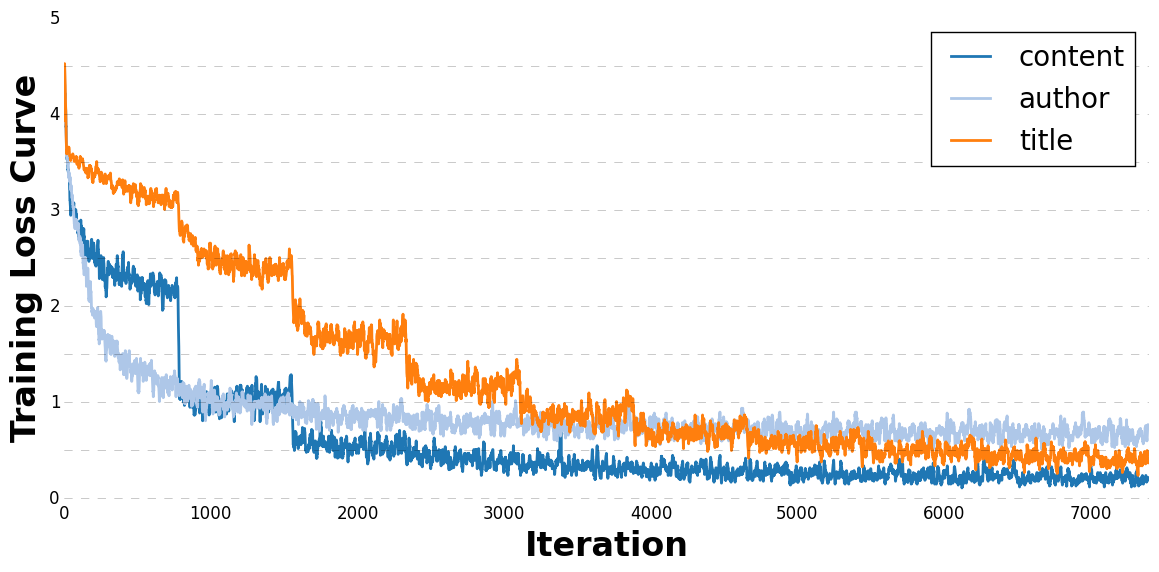
\includegraphics[width=5in]{figures/loss_training_single.png}
\end{center}
\caption{Training loss and testing loss of single LSTM networks.}
\label{training_loss_single}
\end{figure}


\begin{figure}[!t]
\begin{subfigure}{1\textwidth}
  \centering
   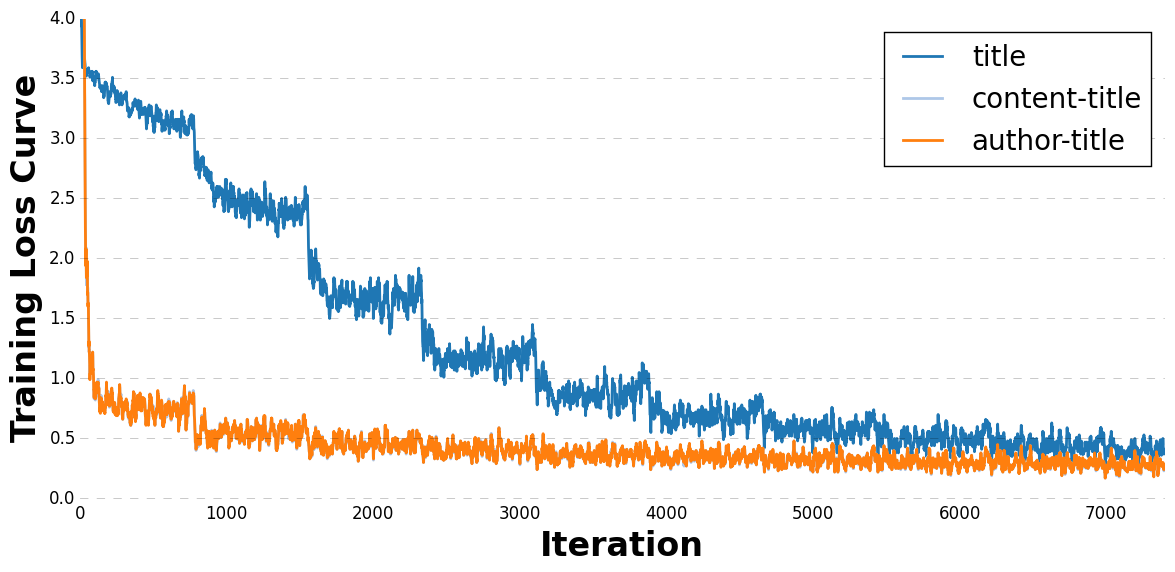
\includegraphics[width=4in]{figures/loss_training_title_modular.png}
   \caption{}
   \label{modular_loss_title}
\end{subfigure}

\begin{subfigure}{1\textwidth}
  \centering
   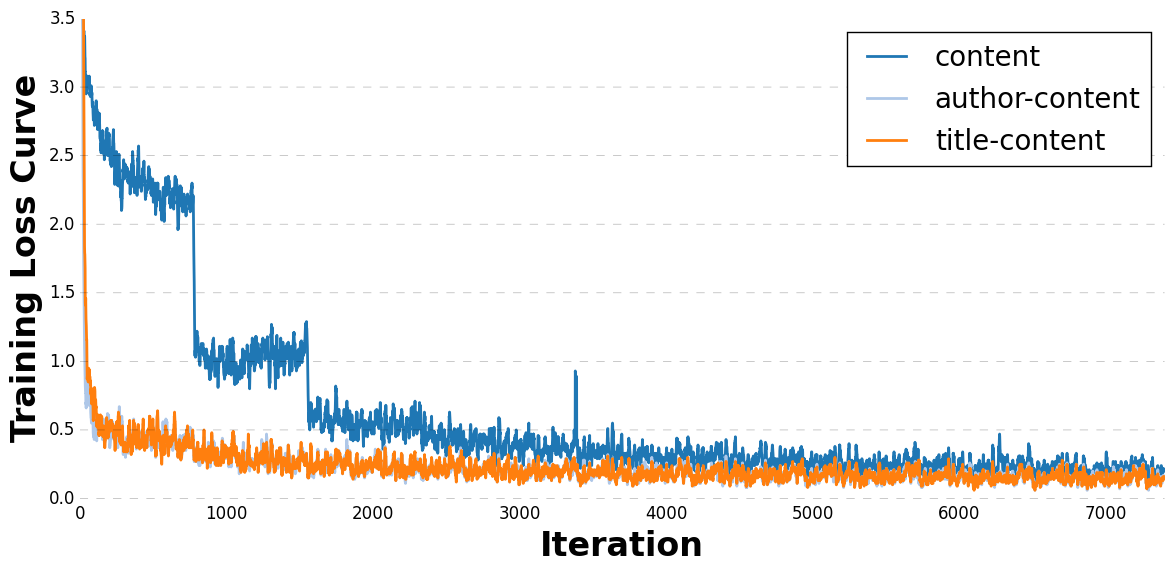
\includegraphics[width=4in]{figures/loss_training_content_modular.png}
   \caption{}
   \label{modular_loss_title}
\end{subfigure}

\begin{subfigure}{1\textwidth}
  \centering
   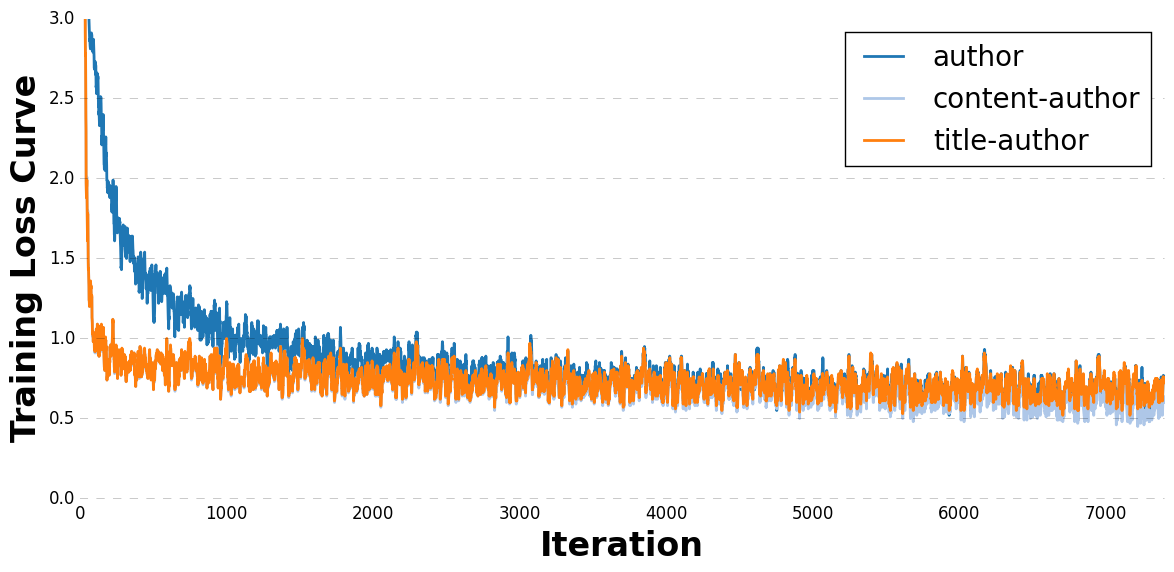
\includegraphics[width=4in]{figures/loss_training_author_modular.png}
   \caption{}
   \label{modular_loss_title}
\end{subfigure}

\caption{Training loss and testing loss of modular LSTM networks: (a) title model based modular LSTM; (b) content model based modular LSTM; (c) author based modular LSTM. In the legends content-title author-title, and etc., the previous one denotes base data source and latter one denotes added data source.}
\label{modular_loss}
\end{figure}

\subsection{Modular LSTM network}

In order to further improve the classification performance, new sources of training data are added to the base single LSTM network. For each single LSTM network, one new data source is added to it, respectively. For example, for content LSTM network, author of the articles and title of the articles are added to it as an additional source of training data. Technically, a new encoder is added to the original LSTM network. The training parameters are same as above. Performance of these modular LSTM networks are reported in Table.\ref{modular_lstm_acc}.

Experimental results show that our modular LSTM networks can effectively exploit new data source in most of the cases. For the author model, which is trained using only author of articles, the classification accuracy has been improved by 0.57\%. One interesting finding is that after adding a new data source to content model, the classification is decreased by 0.34\% and 1.31\%. We can also find that the content-author model \footnote{author is the based data source and content is the added data source} has a much better performance than author-content model. That's because the single author model has a better performance than the single content model, which demonstrates that a good initial model is very crucial in modular LSTM networks.


\begin{table}[!t]
\begin{center}
\caption{Classification performance of modular LSTM networks}
\label{modular_lstm_acc}
\begin{tabular}{c|cc|cc|cc}
\hline

Base source & \multicolumn{2}{c}{Title} & \multicolumn{2}{c}{Content} & \multicolumn{2}{c}{Author} \\
\hline
New source   &   Content   &   Author     &       Title  & Author                &            Content & Title \\
\hline
Training accuracy (\%)   & 95.59  &   95.51    &   97.12   &   97.13    &  86.48  & 85.79\\
Testing accuracy (\%)   &  21.69  &     21.64   &   42.37  &    43.34   &  \textbf{74.46}    & 74.04\\
\hline
Improvement (\%) &           0.46 &     0.41     &      -1.31    &    -0.34  &   \textbf{0.57}   & 0.15 \\

\hline

\hline
\end{tabular}
\end{center}
\end{table}
   

Moreover, the training behavior of them are presented in Fig.\ref{modular_loss}. The  training loss of initial single LSTM and modular LSTM networks are compared with each other. From Fig.\ref{modular_loss} we can see that, in all three cases, after a new data source is added the training loss can converge to a local optimal very fast and the loss values accordingly decrease rapidly. Once a new data source is added, the whole training process can finish in less than 1,000 iterations (near 2 epochs). This demonstrates the efficiency of our MDED network.


\section{Discussion}\label{discussion}
The results of the baseline system for each modality by themselves show significant improvement over the random baseline. We asses that the author modality to be more informative for classification as expected due to low overlap of author names across journals. In addition to the improved accuracy and fast convergence of the system, further improvement in the computational time could be gained by avoiding the optimization step of the trained encoders. In fact, in this paper we only cancel the effect of adaptive gradient descent on the baseline encoder by setting the gradients to zero, but the computations are still carried out. This improvement could be included in frameworks that take advantage of MDEDs for transfer learning.

In future work, more informative evaluation metrics in terms of F1-score and AUC will be provided for better reflection of performance of each system. We plan to also analyze the per class performance. We expect classes with less samples to be less accurate during classification because of data sparsity, which could be solved by discarding the classes with low sample counts thereby increasing the overall accuracy of the system. 

In future work, we would like to apply the concept to other databases and pose the concept to solve inter-database learning. We could also prove the concept in other areas like speech, image and other signal processing domains.

\bibliography{reference} 
\bibliographystyle{ieeetr}

\newpage
\section{Labor Division}
\begin{itemize}
\item
  \textbf{Cheng:} \textbf{Coding} - Data retrieval, unzipping, reading, unicode decoding; \textbf{Report Writing} - Corpora, Evaluation.
\item
  \textbf{Quiangui:} \textbf{Coding} - Core model and augmented model training, Data partitioning, Word2vec model, Training log parsing, Hyper-parameter tuning, Model training, Makefiles. \textbf{Report Writing} - Abstract, Introduction, Hyper-parameter tuning, Results.
\item
  \textbf{Prashanth:} \textbf{Coding} - Data pre-processing, Data partitioning,  Feature representation for embedding layer, Baseline system; \textbf{Report Writing} - Data pre-processing and features, Embedding Layer, Baseline System, Hyper-parameter tuning, Evaluation, Discussion.
\item
    \textbf{Sébastien:} \textbf{Coding} - Core and augmented model definition, experimental results; \textbf{Report Writing} - Proposal, Presentation, Abstract, Introduction, Proposed System, Discussion.
\end{itemize}
\section{Word Count}
\begin{itemize}
\item
109 Abstract
\item
392 Introduction
\item
254 Materials
\item
757 Procedure
\item
126 Evaluation
\item
60 Results: Baseline System
\item
92 Results: Modular LSTM network
\item
224 Discussion
\item
2034 Total
\end{itemize}
%\end{multicols}
\end{document}
